\section{Overall description}
\label{sect:overalldescription}

%\begin{sidewaysfigure}
%\centering
%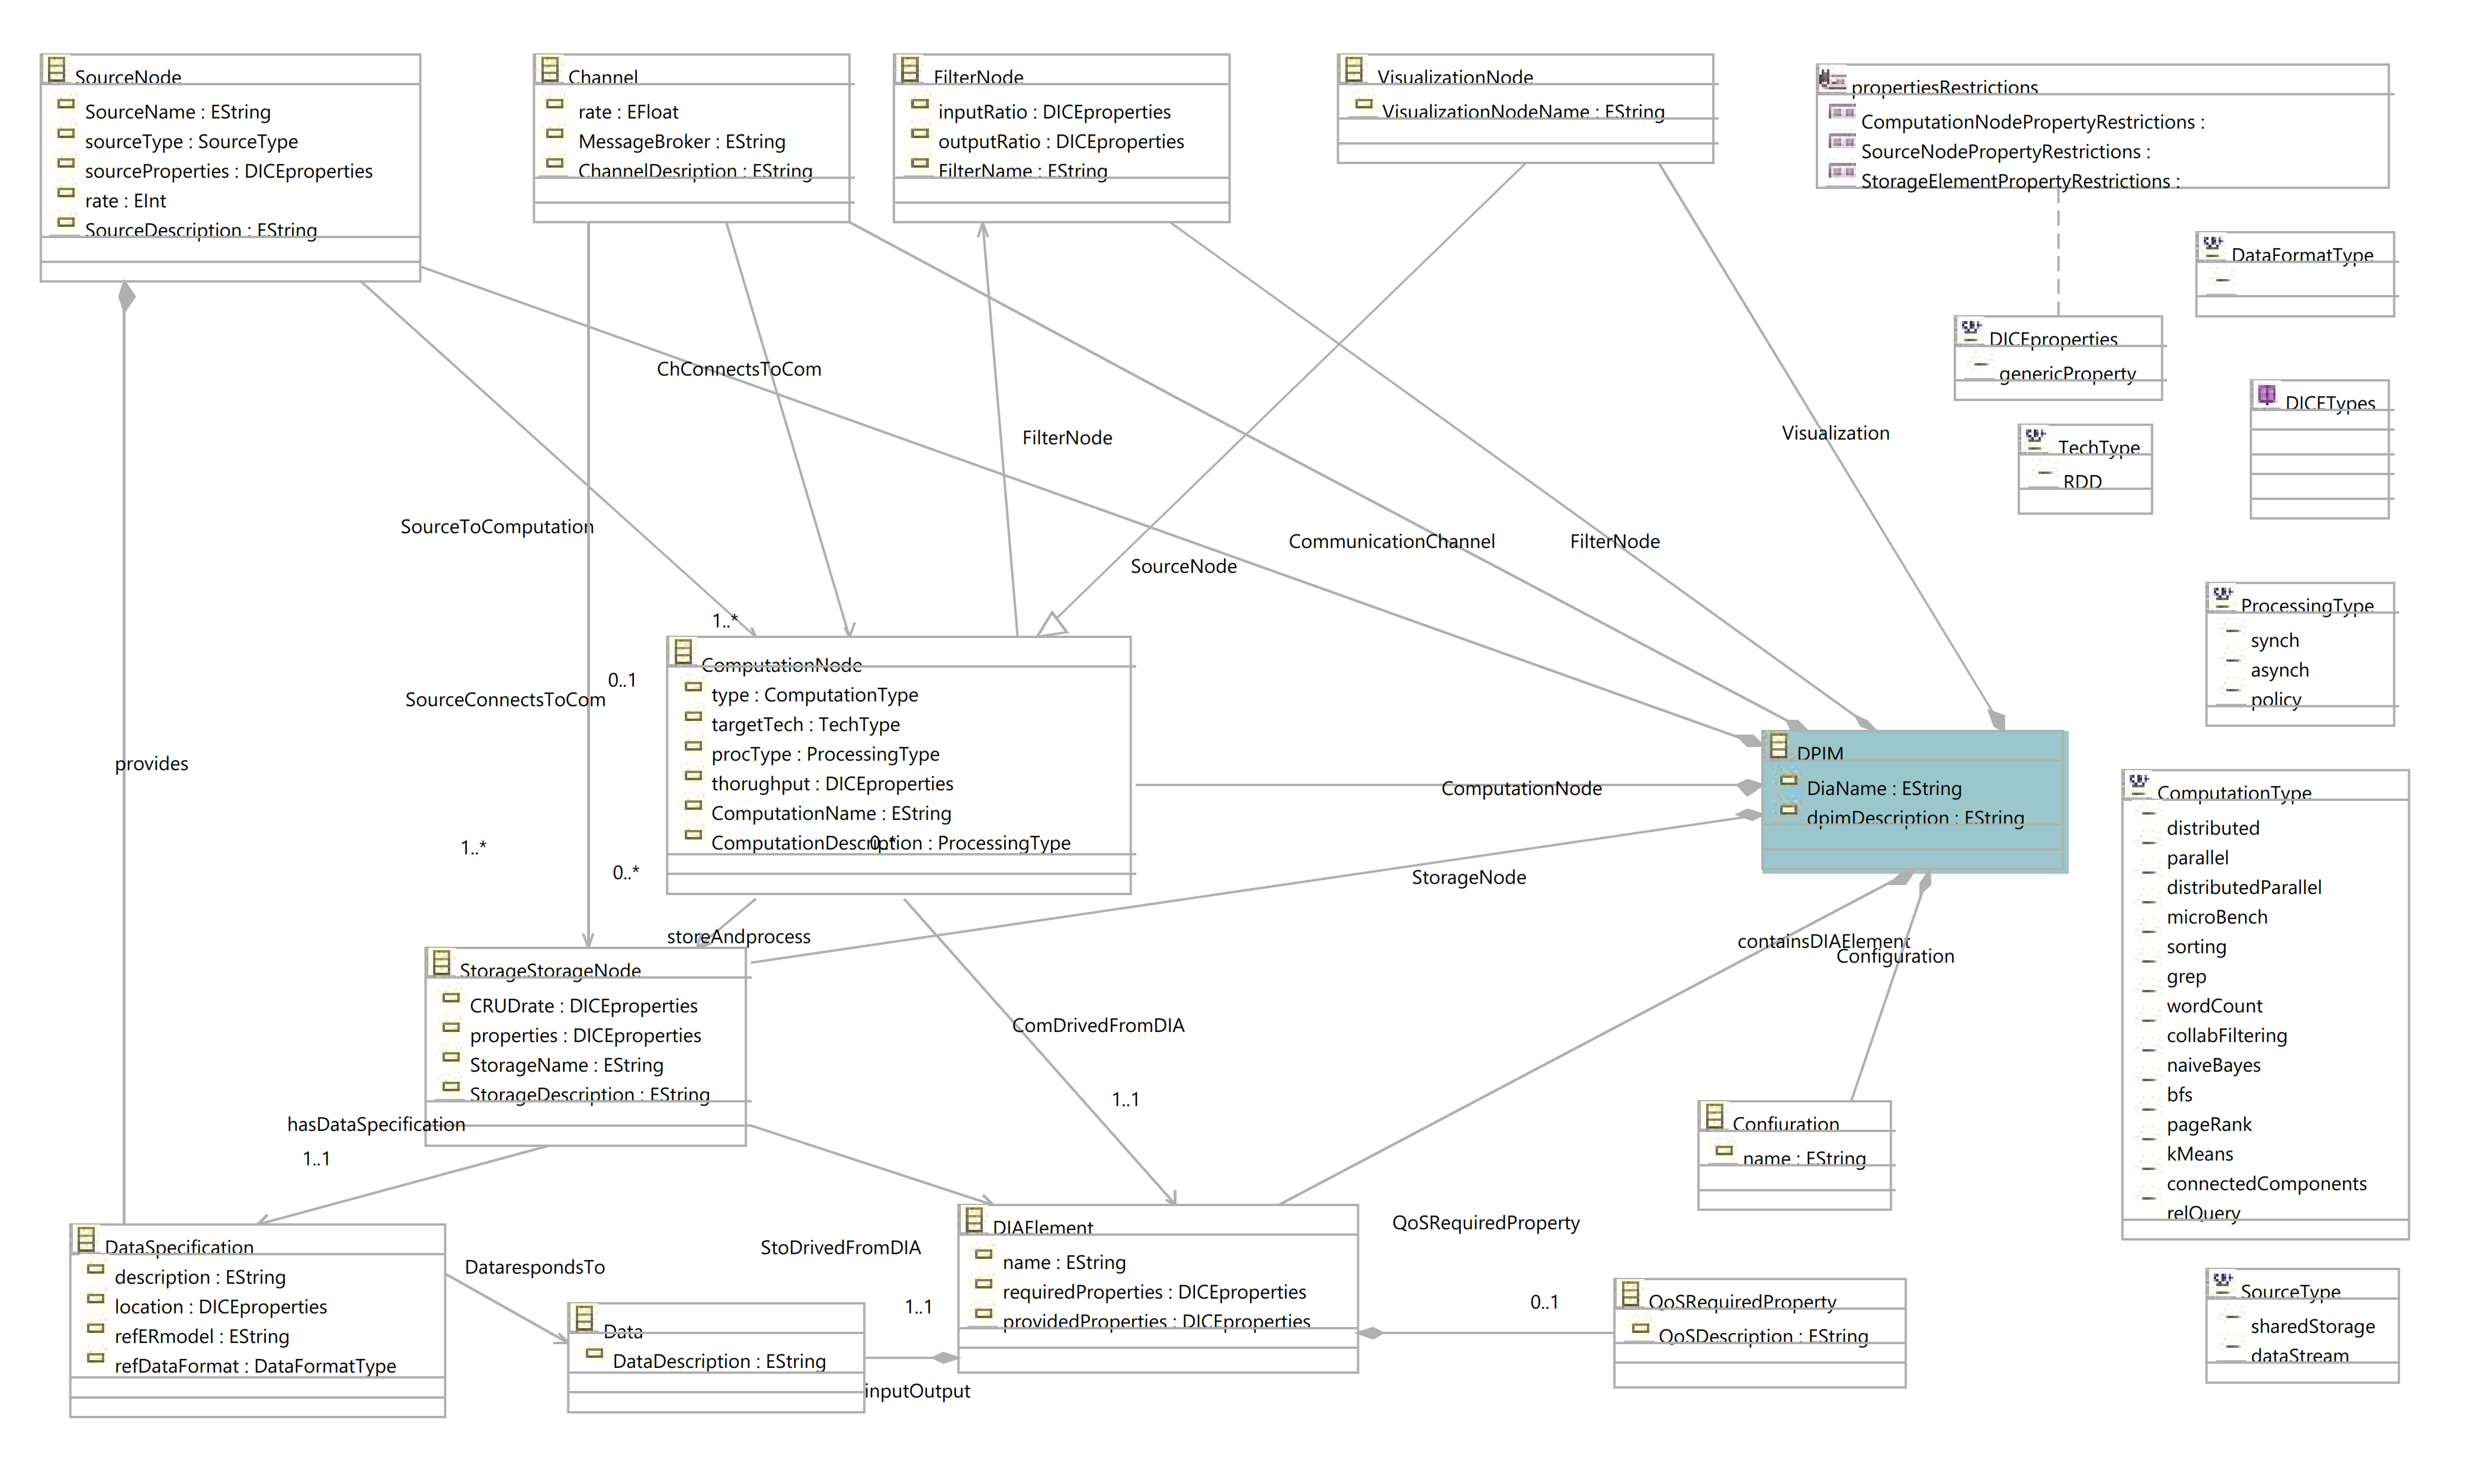
\includegraphics[width=\textwidth]{Images/11.png}
%\caption{\label{fig:metamodel}DICE DPIM metamodel.}
%\end{sidewaysfigure}

%\begin{figure}
%\centering
%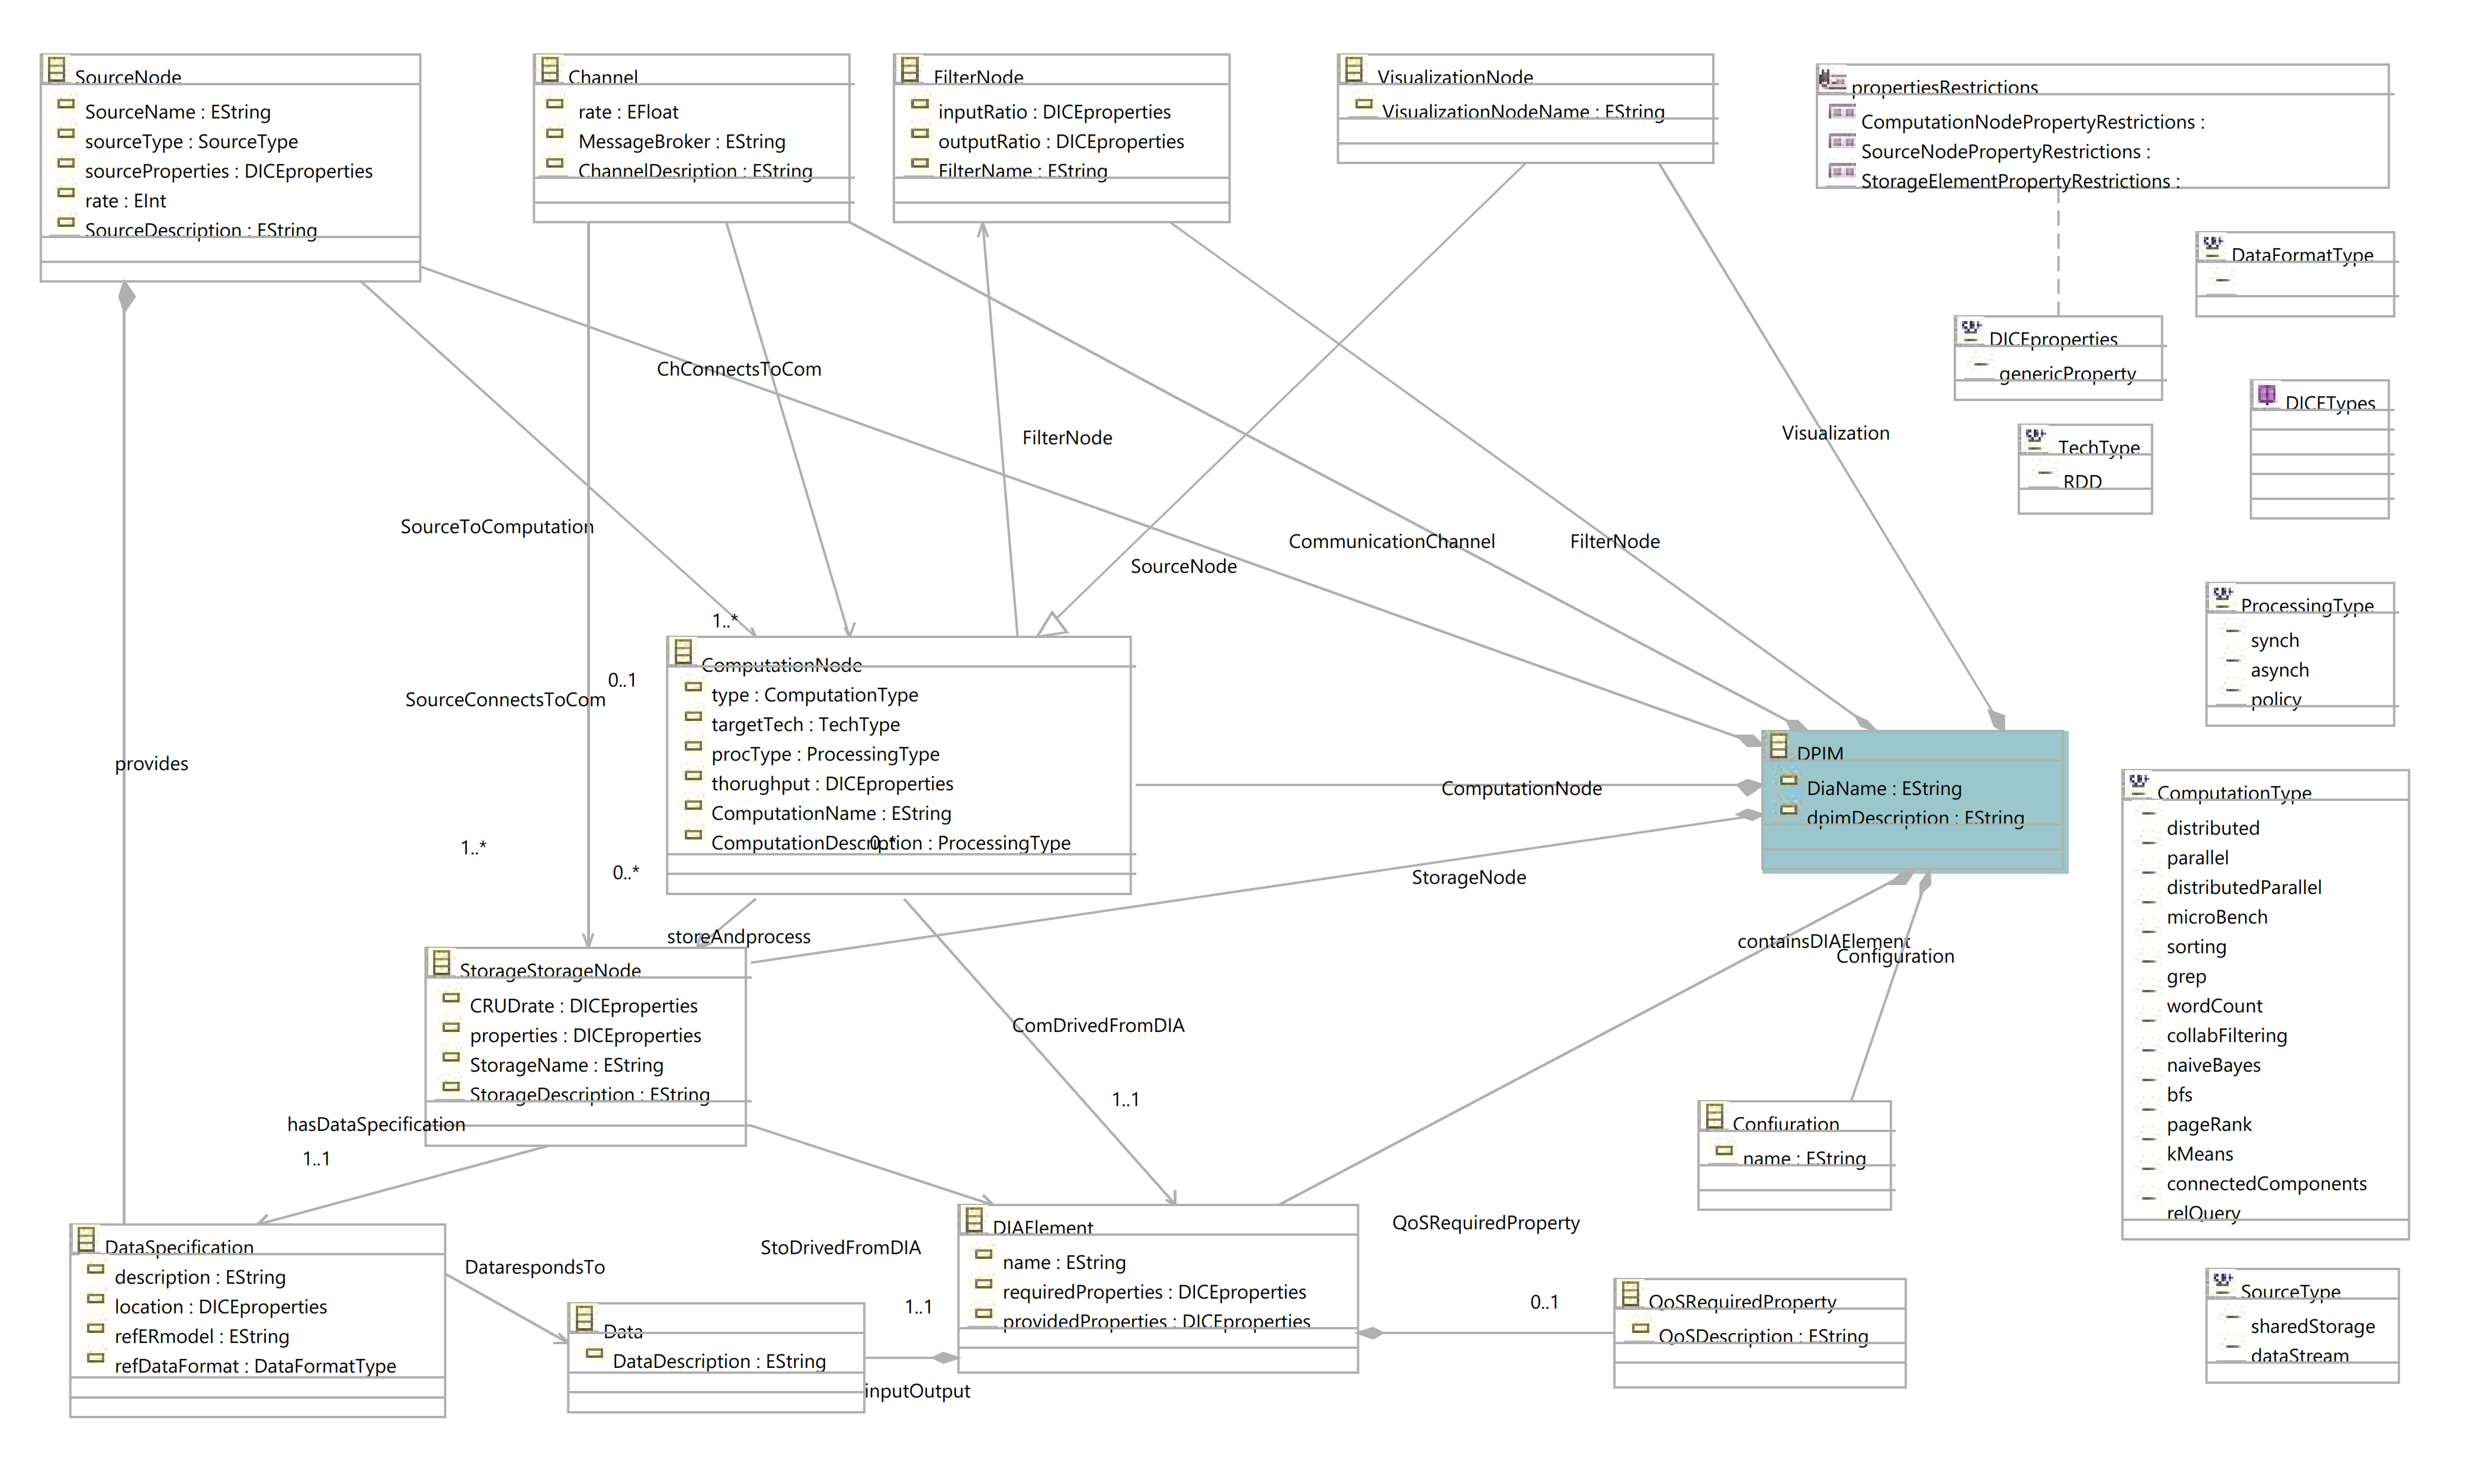
\includegraphics[width=\textwidth]{Images/11.png}
%\caption{\label{fig:metamodel2}DICE DPIM metamodel in portrait form.}
%\end{figure}

\subsection{Goals}
\label{subsect:goals}

The following table shows in details all the main goals that our application wants to meet. 

We managed to divide them in two main categories: goals related to the shop owners and goals related to the clients. Also, we have assigned an unique identifier to each one of them in order to be able to refer to them later in the document.

\begin{table}[h!]
    \centering
    \begin{tabular}{@{}P{0.1\textwidth}P{0.80\textwidth}@{}}
        \multicolumn{2}{c}{\textbf{Shop owners}} \\
        \toprule
        \textbf{Identifier}& \textbf{Goal}\\
        \midrule
        \textbf{G1}        & Allow manager to sign on the system\\
        \textbf{G2}        & Allow a manager to sign in the system\\
        \textbf{G3}        & Allow a manager to register their store/stores on the system\\
        $\;\;$    G3.1  & Allow a manager to register basic info about the shop\\
        $\;\;$    G3.2  & Allow a manager to divide their store in areas \\
        $\;\;$    G3.3  & Allow a manager to register the items in the areas \\
        \textbf{G4}        & Allow a manager to update the shop info\\
        \textbf{G5}        & Allow a manager to check the general status of their shop\\
    \end{tabular}
\caption{Shop owner's goals}
\label{table:shopownersgoals}
\end{table}

\begin{table}[h!]
    \centering
    \begin{tabular}{@{}P{0.1\textwidth}P{0.80\textwidth}@{}}
        \multicolumn{2}{c}{\textbf{Clients}} \\
        \toprule
        \textbf{Identifier}& \textbf{Goal}\\
        \midrule
        \textbf{G6}        & Allow a customer to join the virtual queue from the spot\footnotemark\\
        \textbf{G7}        & Allow a user to sign on the system\\
        \textbf{G8}        & Allow a user to sign in the system\\
        \textbf{G9}        & Allow a user to join the virtual queue from the app\\
        \textbf{G10}       & Allow a user to book a shopping session at a grocery store\\
        $\;\;$    G10.1 & Allow a user to select the time and duration(between predefined options) for they session\\ 	
        $\;\;$    G10.2 & Allow a user to select categories of items they are willing to buy\\
        \textbf{G11}       & Allow a user to retrieve informations about its previously booked visits\\
        \textbf{G12}       & Allow a user to retrieve informations about the congestion of shops\\
        \textbf{G13}       & Allow a customer to use a QR code to get access to the store \\
        \bottomrule
    \end{tabular}
\caption{Client's goals}
\label{table:clientsgoals}
\end{table}
\footnotetext{with the facility of a hardware support, it will be better specificed later on this document.}

\subsection{Domain Assumptions}
\label{subsect:domainassumptions}

The following table list all the assumptions over which we cannot have control, but we assume as verified.

As with the goals in the section above, we provide them with an unique identifier to keep track of them in the document.

\begin{table}[h!]
    \centering
    \begin{tabular}{@{}P{0.1\textwidth}P{0.80\textwidth}@{}}
        \toprule
        \textbf{identifier}& \textbf{Domain Assumption}\\
        \midrule
        \textbf{D1}        & Data provided from GPS is valid and accurate\\
        \textbf{D2}        & Google Maps' paths calculator makes correct time estimations\\
        \textbf{D3}        & A person cannot get in the store without having scanned the QR code\\
        \textbf{D4}        & A person cannot get out of the store without having scanned the QR code\\
        \textbf{D5}        & The number of people entering the store is coherent with the data related to the QR code scanned\\
        \textbf{D6}        & Each store registered on the system is provided with the necessary functioning hardware\\
        \textbf{D7}        & Data provided from managers is legit\\
        $\;\;$D7.1         & Managers provide the maximum number of person allowed in the store by the law (non penso sia da mettere, non è di nostro interesse che questo dato sia corretto secondo la legge. L'unica cosa che ci interessa è che questo dato venga inserito per forza, e possiamo occuparcene obbligando il manager a scriverlo al momento della registrazione del negozio)\\
        $\;\;$D7.2         & Managers will provide the correct number of people that can be in a group togheder shopping by the law (stessa nota di sopra)\\
        $\;\;$D7.3         & Managers will provide the correct address of their store\\
        $\;\;$D7.4         & Managers will provide the correct schedule of their store\\
        $\;\;$D7.5         & Managers will provide the correct categories of items they sell\\
        $\;\;$D7.6         & Managers will map the categories of items in the correct areas of the shop (non ne sono ancora convinto, mi spiace.. Domani ne riparliamo)\\
        $\;\;$D7.7         & Managers will correctly map items with the respective category\\
        \textbf{D8}       & Areas of the shop don’t overlap\\
        \textbf{D9}       & A customer will take the shortest path to the store when they receive the notification (anche questo non mi sembra proprio una domain assumption, però la lascerei)\\
        \textbf{D10}       & Customers will stay in the store approximately the time they have claimed they would\\
        \textbf{D11}       & Customers will shop the items they have claimed they would\\
        \textbf{D12}       & Phone number are unique\\
        \textbf{D13}       & Emails are unique\\
        \textbf{D14}       & Notification sent to the users, may them be managers or clients, will be surely received and comprehended by them\\
        \textbf{D15}       &  people are not malicious against the app (well, problem solved. lol... )\\
        \textbf{D16}       & Managers' emails are correctly validated by PEC system\\
        \textbf{D17}       & Users are aware of the process required to scan a QR code\\
        \bottomrule
    \end{tabular}
\caption{Domain assumptions}
\label{table:domainassumptions}
\end{table}

\subsection{Constraints}
\label{subsect:contraints}

Constraints: imposed by the client or the environment in which the system operates. 

Anything that will limit the developer’s options (e.g. regulations, reliability, criticality, hardware limitations, parallelism, etc.)

\subsubsection{Regulatory policies}
\label{subsubsect:regulatorypolicies}

\begin{itemize}
    \item ask user permission to retrieve and use GPS data
    \item Telephone numbers and emails will not be used for commercial purpose
    \item respect privacy law about user data
    \item Managers can access only to anonymous data about user's booked visits or enqueued clients
    \item 
\end{itemize}

\subsubsection{Hardware limitations}
\label{subsubsect:hardwarelimitations}

\begin{itemize}
    \item Mobile app (requires a smartphone with internet connection and GPS, either android or ios)
    \item Web app (requires a modern browser able to retrieve user location and with an internet connection)
    \item QR scanner (able to scan QR codes and with an internet connection in order to communicate with our servers)
    \item Turnstile (connected with the QR scanner)
\end{itemize}


\subsubsection{Interfaces to other applications}
\label{subsubsect:interfacestootherappications}

\begin{itemize}
    \item GPS
    \item Google Maps
    \item QR scanners API (?)
    \item turnstile API (?)
\end{itemize}

\subsection{Product perspective}
\label{subsect:productperspective}

Here we include scenarios and further details on the shared phenomena and a domain model (class diagrams and statecharts).

Describes external interfaces: system, user, hardware, software; also operations and site adaptation, and hardware constraints

\subsubsection{scenarios}
\label{subsubsect:scenarios}

In this section we want to present some usefull scenarios to better describe what people will do and experience as they try to make use of CLup services. Our intent is not to specify every possible situation, but to give the reader a general understanding of the main features of the system with a concrete description of ideal cases.
 
\begin{description}
    \item[User lines up] 
    In a period of global pandemic and quarantine, XXX needs to do the grocery shopping and, remembering the risks he used to take when there was no organization, he smiles opening the CLup app from his smatphone. He immediately searches the store he wants to go to, and in a few clicks he has all the relevant information about the status of the virtual queue and an estimation of how much time to wait. He decides to enqueue himself and by informing the app about his stay at the shop and how he'll reach it, he's ready to confirm and receive his personal QR code. Now it's time for XXX to wait in the comfort of his house, untill, when the time comes, he receives a push(?) notification from the app telling him that it is the right moment to head towards his destination. When he arrives he finds no queue outside the store, and, by simply scanning his QR code, he's able to enter and exit the shop in a safe and controlled environment.

    \item[Customer lines up]
    As every monday, even this monday Mr. ZZZ goes to the nearby supermarket to gather all he needs for the week. He is used to wait for his turn standing outside in a queue and for someone of his age it's not a simple task. Approaching the entrance of the store he is really surprised noticing that there is no queue, and, rushing inside, he sees a new installation blocking his way: a turnstile and a ticket machine next to it. He reads all the new rules to follow and immediately after he clicked a few button on the new machine, he receives a ticket with the time he needs to wait to enter printed. Now Mr.ZZZ can safely wait his turn while sitting on the beneches of the nearby park. When his time will come he'll be able to enter and exit the store scanning the ticket at the turnstile.

    \item[User books a visit]
    YYY has a really strict and rigid work schedule and lately he has found himself unable to go grocery shopping, because of long queues and closing hours of supermarkets. Luckily for him, one of his co-worker tells him that CLup app has a "book a visit" features to better help people manage their time. YYY decides to try it and, after downloading the app and signing up, he searches the store he needs to go to, checks the available reservations, and books the one right after work. The very next day at 7 p.m., when everybody is leaving the office, YYY receives a remainder from the CLup application about his reservation: he will no longer waste a minute in queues neither he'll be left without being able to do the shopping.

    \item[Manager registers a shop]
    During quarantine shops are subjected to strict rule in order to guarantee health safety to their clients. WWW has dealt with a lot of legal problem during the first months of the quarantine, because of how difficoult it can be to regulate and monitor traffic through all of his shops. This time he has decided to turn to CLup to precisely regulate the flow of customers and to avoid any problem with crowd forming inside or outside his shops. First of all he visited CLup website and by registering as manager... ?

    \item[Manager updates shop's info]
    The pandemic is unpredictable and therefore sometimes WWW finds himself having to close his supermarket, or changing some parameters beacause of new laws. CLup helps him customize everything he needs to, infact in a few clicks from the app a shop manager can update all the shop's info. For example when... ?
\end{description}


\subsubsection{Use cases}
\label{subsubsect:usecases} 

Here we generalize scenarios. Keep use cases small (no more than two/three pages).
Srtucture the description in terms of:
\begin{itemize}
    \item use case name: verb that indicate what the user is trying     to accomplish;
    \item participating actors;
    \item entry condition;
    \item flow of events: The steps accomplished by actors and those accomplished by the system should be clearly distinguished and the causal relationship between steps should be clear;
    \item exit condition;
    \item exceptions;
    \item special requirements (constraints, nonfunctional requirements).
\end{itemize}



\subsubsection{Class diagrams and statecharts}
\label{subsubsect:diagrams}

What should we model? The objects and people that are of interest for the given problem. The relevant phenomena. The goals, requirements, and domain assumptions.

How do we find objects? Analyze any description of the problem, the application domain, the scenarios and use cases. 

to model dynamic behavior of a single object we use state machine diagram.

From the flow of events in the use case or scenario, proceed to the sequence diagram. A sequence diagram is a graphical description of objects participating in a use case or scenario using a DAG (directed acyclic graph) notation.

Consider using state diagrams and activity diagrams.

What is the structure of the world? $\rightarrow$ Create class siagrams for static information models (UML). Is there any state change in an object that is to be defined explicitly? $\rightarrow$ Create state diagrams for dynamic class behavior models. How is the expected interaction between the software to be and the environment? Create sequence diagrams from use cases for dynamic object behavior instance examples; or create activity diagrams when you want to highlight important process.

UML does not help us in expressing assertions, we can complement its usage with some formal or informal description of these assertions.

\subsection{Product functions}
\label{subsect:productfunctions}

Here we include the most important requirements.

\subsection{User characteristics}
\label{subsect:usercharacteristics}

Here we include anything that is relevant to clarify their needs.

\subsubsection{Actors}
\label{subsubsect:actors}

Customer: a person who grocery shops.
user: a customer using Clup and who is registered on the system. They can join the virtual queue, book a shopping session and ask/receive updates.
Shop manager: a person who register their shop on Clup. A shop manager can register multiple shop on the system.
Shop: a grocery shop registered on the system. It updates periodically the people present in the store and sends updates to the manager.

\subsection{Phenomena [sezione provvisoria]}
\label{subsect:phenomena}

The machine: the portion of system to be developed.
The world (a.k.a. the environment): the portion of the real-world affected by the machine.
Requirements engineering is concerned with phenomena occurring in the world, as opposed to phenomena occurring inside the machine.

Goals are prescriptive assertions formulated in terms of \textbf{world} phenomena (not necessarily shared).
Domain properties/assumptions are descriptive assertions assumed to hold in the \textbf{world}.
Requirements are prescriptive assertions formulated in terms of \textbf{shared} phenomena.
Requirements are a bridge from the \textbf{machine} to the real \textbf{world}.

Find all the possible phenomena, for each one specify if its shared or not and who controls it (world or machine). 

\subsubsection{World phenomena}
\label{subsubsect:worldphenomena}

World phenomena are phenomena that the machine can not observe.

\subsubsection{Shared Phenomena}
\label{subsubsect:sharedphenomena}

Some world phenomena are shared with the machine.
Shared phenomena can be controlled by the world and observed by the machine, or controlled by the machine andd observed by t5he world.
